\chapter{Conception et réalisation de l'application}
\section{Introduction}
Dans ce chapitre, nous allons présenter l'environnement de travail et les choix architecturaux. En premier lieu, nous parlerons de l'environnement matériel et logiciel. Après, nous proposerons nos choix architecturaux.
\section{Environnement de travail}
Cette section va être dédiée à la présentation de l'environnement de travail que ce soit matériel ou logiciel.
\subsection{Environnement matériel}
Le tableau \ref{code20} présente les caractéristiques techniques de la machine utilisé.
\begin{table}[H]
\centering
\caption{Caractéristiques techniques de la machine}
\label{code20}
\begin{tabular}{|l|l|}
\hline
\textbf{Constructeur} & Dell Inc. \\
\hline
\textbf{Processeur} & Intel(R) Core(TM) i3-2100 CPU @ 3.10GHz \\ \hline
\textbf{RAM} & 8.0 GO \\ \hline
\textbf{Disque dur} & 500.0 GO \\ \hline
\textbf{Système d'exploitation} & Microsoft Windows 10 Entreprise (x64) \\ \hline
\end{tabular}
\end{table}
\subsection{Environnement logiciel}
Dans cette partie, nous allons présenter les logiciels utilisés en plus des technologies.
\subsubsection{Eclipse}
\noindent\begin{minipage}{0.69\textwidth}
Eclipse est un environnement de développement intégré qui est open source. Cet outil a été utilisé pour développer la partie back-office \footnotemark de l'application qui est en Java.
\end{minipage}
\footnotetext{Back-office désigne les applications qui ne sont pas accessibles au client final}
\begin{minipage}{0.3\textwidth}
\begin{figure}[H]
  \centering
  
\includegraphics[scale=0.6]{figures/logo/eclipse.png}
  \caption{Logo Eclipse}
  \label{code21}
\end{figure}
\end{minipage}
\subsubsection{Sublime Text 3}
\noindent\begin{minipage}{0.69\textwidth}
Sublime Text 3 est un éditeur de texte qui facilite la saisie de code grâce à son auto-complétion, aux différents raccourcis et à la coloration de syntaxe. Cet outil a été utilisé pour développer la partie front-office \footnotemark de l'application qui est en Javascript, HTML et CSS.
\end{minipage}
\footnotetext{Front-office désigne les applications accessibles au client final}
\begin{minipage}{0.3\textwidth}
\begin{figure}[H]
  \centering
  
\includegraphics[scale=0.25]{figures/logo/Sublime_Text_3.png}
  \caption{Logo Sublime Text}
  \label{code22}
\end{figure}
\end{minipage}
\subsubsection{Oracle SQL Developer}
\noindent\begin{minipage}{0.69\textwidth}
Oracle SQL Developer est environnement de développement intégré permettant d'interroger les bases de données Oracle grâce au langage SQL. Cet outil a été utilisé pour consulter la base de données distante de l'application Jira en plus de la base de données de notre application.
\end{minipage}
\begin{minipage}{0.3\textwidth}
\begin{figure}[H]
  \centering
  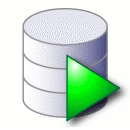
\includegraphics[scale=0.5]{figures/logo/orclsqldev3.jpg}
  \caption{Logo Oracle SQL Developer}
  \label{code23}
\end{figure}
\end{minipage}
\subsubsection{Edraw Max}
\noindent\begin{minipage}{0.69\textwidth}
Edraw Max est un logiciel permettant de créer des diagrammes de toutes sortes. Ce logiciel a été utilisé pour la création de l'organigramme de la société.
\end{minipage}
\begin{minipage}{0.3\textwidth}
\begin{figure}[H]
  \centering
  
\includegraphics[scale=0.25]{figures/logo/edraw_max.png}
  \caption{Logo Edraw max}
  \label{code24}
\end{figure}
\end{minipage}
\subsubsection{Enterprise Architect}
\noindent\begin{minipage}{0.69\textwidth}
Enterprise Architect est un logiciel permettant de créer des diagrammes UML. Ce logiciel a été utilisé pour la conception de notre application afin de créer les diagrammes UML utilisés dans le rapport.
\end{minipage}
\begin{minipage}{0.3\textwidth}
\begin{figure}[H]
  \centering
  
\includegraphics[scale=0.3]{figures/logo/enterprisearchitect.png}
  \caption{Logo Enterprise Architect}
  \label{code25}
\end{figure}
\end{minipage}
\subsubsection{Google Chrome}
\noindent\begin{minipage}{0.69\textwidth}
Google Chrome est un navigateur web disposant d'une console permettant de debug le code de notre application front-office. Cet outil a été utilisé pour la visualisation de l'application web.
\end{minipage}
\begin{minipage}{0.3\textwidth}
\begin{figure}[H]
  \centering
  
\includegraphics[scale=0.2]{figures/logo/chrome.png}
  \caption{Logo Google Chrome}
  \label{code26}
\end{figure}
\end{minipage}
\subsubsection{Postman}
\noindent\begin{minipage}{0.69\textwidth}
Postman est une application permettant de tester les services web. Cette application a été utilisé pour tester tous les services web de notre application back-office.
\end{minipage}
\begin{minipage}{0.3\textwidth}
\begin{figure}[H]
  \centering
  
\includegraphics[scale=0.12]{figures/logo/postman.png}
  \caption{Logo Postman}
  \label{code27}
\end{figure}
\end{minipage}
\subsubsection{Overleaf}
\noindent\begin{minipage}{0.69\textwidth}
Overleaf est un éditeur de rapport Latex en ligne. Il dispose d'outil de gestion de version en plus de sa facilité d'utilisation. Cet outil a été utilisé pour éditer le rapport de notre projet de fin d'études.
\end{minipage}
\begin{minipage}{0.3\textwidth}
\begin{figure}[H]
  \centering
  
\includegraphics[scale=1]{figures/logo/overleaf.png}
  \caption{Logo Overleaf}
  \label{code28}
\end{figure}
\end{minipage}
\subsubsection{Sharelatex}
\noindent\begin{minipage}{0.69\textwidth}
Sharelatex est aussi un éditeur de rapport Latex en ligne. En plus de sa facilité d'utilisation, ce dernier n'a pas de limitations si vous allez l'utiliser sans collaborateurs. Cet outil a été utilisé pour éditer le rapport de notre projet de fin d'études.
\end{minipage}
\begin{minipage}{0.3\textwidth}
\begin{figure}[H]
  \centering
  
\includegraphics[scale=0.25]{figures/logo/sharelatex.jpg}
  \caption{Logo Sharelatex}
  \label{code52}
\end{figure}
\end{minipage}
\subsubsection{Trello}
\noindent\begin{minipage}{0.69\textwidth}
Trello est un outil de gestion de projet en ligne. Nous l'avons utilisé pour gérer les sprints de notre projet.
\end{minipage}
\begin{minipage}{0.3\textwidth}
\begin{figure}[H]
  \centering
  
\includegraphics[scale=0.3]{figures/logo/trello.png}
  \caption{Logo Trello}
  \label{code29}
\end{figure}
\end{minipage}
\subsubsection{Ollert}
\noindent\begin{minipage}{0.69\textwidth}
Ollert est un outil de génération de rapports sur l'avancement d'un projet géré par Trello. Cet outil a été utilisé pour visualiser notre avancement tout au long du projet.
\end{minipage}
\begin{minipage}{0.3\textwidth}
\begin{figure}[H]
  \centering
  
\includegraphics[scale=0.2]{figures/logo/ollert.png}
  \caption{Logo Ollert}
  \label{code30}
\end{figure}
\end{minipage}
\subsubsection{DB Designer}
\noindent\begin{minipage}{0.69\textwidth}
DB Designer est un outil de création d'un schéma de base de données en ligne. Cet outil permet d'exporter le schéma sous format SQL. Nous avons utilisé ce dernier pour pouvoir créer le schéma de base de données de notre application afin de pouvoir en discuter lors des réunions hebdomadaires.
\end{minipage}
\begin{minipage}{0.3\textwidth}
\begin{figure}[H]
  \centering
  
\includegraphics[scale=1]{figures/logo/db_designer.png}
  \caption{Logo DB Designer}
  \label{code31}
\end{figure}
\end{minipage}
\subsubsection{Jira}
\noindent\begin{minipage}{0.69\textwidth}
Jira est un outil de gestion de projet piloté par Scrum ou Kanban \footnotemark. Cet outil est utilisé dans la société pour piloter les projets et sa base de données contient des informations sur les employés de cette dernière. Nous avons utilisé Jira pour pouvoir en extraire les données sur les employés afin de calculer les indicateurs de performance.
\end{minipage}
\footnotetext{C'est une méthode de travail japonaise connu pour son efficacité dans la gestion de projet}
\begin{minipage}{0.3\textwidth}
\begin{figure}[H]
  \centering
  
\includegraphics[scale=0.3]{figures/logo/jira.jpg}
  \caption{Logo Jira}
  \label{code32}
\end{figure}
\end{minipage}
\subsubsection{Apache Tomcat}
\noindent\begin{minipage}{0.69\textwidth}
Apache Tomcat est un serveur HTTP et conteneur web libre de servlet \cite{Tomcat}. Cet outil a été utilisé pour héberger notre application back-office.
\end{minipage}
\begin{minipage}{0.3\textwidth}
\begin{figure}[H]
  \centering
  
\includegraphics[scale=0.17]{figures/logo/tomcat.png}
  \caption{Logo Apache Tomcat}
  \label{code33}
\end{figure}
\end{minipage}
\subsubsection{Yeoman}
\noindent\begin{minipage}{0.69\textwidth}
Yeoman est un générateur de code utilisé pour générer des projets web. Cet outil a été utilisé pour générer le squelette initial de notre application web en plus des composants de cette dernière.
\end{minipage}
\begin{minipage}{0.3\textwidth}
\begin{figure}[H]
  \centering
  
\includegraphics[scale=0.17]{figures/logo/yeoman.png}
  \caption{Logo Yeoman}
  \label{code34}
\end{figure}
\end{minipage}
\subsubsection{Dozer}
\noindent\begin{minipage}{0.69\textwidth}
Dozer est un outil de mise en correspondance des données en Java / JEE. Cet outil a été utilisé pour mettre en correspondance les modèles et les entités.
\end{minipage}
\begin{minipage}{0.3\textwidth}
\begin{figure}[H]
  \centering
  
\includegraphics[scale=0.38]{figures/logo/dozer.png}
  \caption{Logo Dozer}
  \label{code35}
\end{figure}
\end{minipage}
\subsubsection{NodeJs}
\noindent\begin{minipage}{0.69\textwidth}
NodeJs est un runtime Javascript permettant d’exécuter du code Javascript côté serveur. Cet outil dispose aussi d'un manager de paquetage Javascript Open Source appelé Npm. Cet outil a été utilisé pour installer différents paquetages pour notre projet front-office.
\end{minipage}
\begin{minipage}{0.3\textwidth}
\begin{figure}[H]
  \centering
  
\includegraphics[scale=0.12]{figures/logo/nodejs.jpg}
  \caption{Logo NodeJS}
  \label{code36}
\end{figure}
\end{minipage}
\subsubsection{Bower}
\noindent\begin{minipage}{0.69\textwidth}
Bower est un manager de paquetage comme Npm. Cet outil a aussi été utilisé pour installer différents paquetages pour notre projet front-office.
\end{minipage}
\begin{minipage}{0.3\textwidth}
\begin{figure}[H]
  \centering
  
\includegraphics[scale=0.17]{figures/logo/bower.png}
  \caption{Logo Bower}
  \label{code37}
\end{figure}
\end{minipage}
\subsubsection{Grunt}
\noindent\begin{minipage}{0.69\textwidth}
Grunt est un outil d'automatisation de code Javascript. Cet outil a été utilisé comme serveur http pour héberger notre application front-office et pour gérer le changement de code.
\end{minipage}
\begin{minipage}{0.3\textwidth}
\begin{figure}[H]
  \centering
  
\includegraphics[scale=0.25]{figures/logo/grunt.png}
  \caption{Logo Grunt}
  \label{code38}
\end{figure}
\end{minipage}
\subsubsection{Maven}
\noindent\begin{minipage}{0.69\textwidth}
Maven est un moteur de production pour les applications Java / JEE. Cet outil a été utilisé pour gérer les dépendances du projet en plus de la génération de codes.
\end{minipage}
\begin{minipage}{0.3\textwidth}
\begin{figure}[H]
  \centering
  
\includegraphics[scale=0.4]{figures/logo/maven.png}
  \caption{Logo Maven}
  \label{code39}
\end{figure}
\end{minipage}
\subsubsection{Hibernate}
\noindent\begin{minipage}{0.69\textwidth}
Hibernate est un ORM \footnotemark servant à la gestion de persistance de la base de données relationnelle. Cet outil a été utilisé pour gérer la base de données de notre application back-office.
\end{minipage}
\footnotetext{Object Relationship Mapping ou en français Mapping objet relationnel est un outil permettant de gérer la persistance des données entre l'application et la base de données relationnelle}
\begin{minipage}{0.3\textwidth}
\begin{figure}[H]
  \centering
  
\includegraphics[scale=0.35]{figures/logo/hibernate.png}
  \caption{Logo Hibernate}
  \label{code40}
\end{figure}
\end{minipage}
\subsubsection{Spring}
\noindent\begin{minipage}{0.69\textwidth}
Spring est un framework Java / JEE conçu pour faciliter le développement d'applications. Ce framework a plusieurs avantages tels que la facilité d'utilisation ou son architecture robuste et facile à comprendre. Ce framework a été utilisé pour développer notre application back-office.
\end{minipage}
\begin{minipage}{0.3\textwidth}
\begin{figure}[H]
  \centering
  
\includegraphics[scale=0.35]{figures/logo/spring.png}
  \caption{Logo Spring}
  \label{code41}
\end{figure}
\end{minipage}
\subsubsection{AngularJS}
\noindent\begin{minipage}{0.69\textwidth}
AngularJS est un framework MVC \footnotemark Javascript conçu pour développer des applications web. Ce framework a été utilisé pour développer notre application front-office.
\end{minipage}
\footnotetext{Model-View-Controller ou en français modéle, vue et contrôleur est une architecture logicielle populaire pour les applications web}
\begin{minipage}{0.3\textwidth}
\begin{figure}[H]
  \centering
  
\includegraphics[scale=0.5]{figures/logo/angularjs.png}
  \caption{Logo AngularJS}
  \label{code42}
\end{figure}
\end{minipage}
\subsubsection{Java}
\noindent\begin{minipage}{0.69\textwidth}
Java est un langage de programmation orienté objet qui permet de développer une application indépendante des architectures logicielles \cite{Java}. Ce langage a été utilisé pour développer l'application back-office.
\end{minipage}
\begin{minipage}{0.3\textwidth}
\begin{figure}[H]
  \centering
  
\includegraphics[scale=0.15]{figures/logo/java.png}
  \caption{Logo Java}
  \label{code43}
\end{figure}
\end{minipage}
\subsubsection{Javascript}
\noindent\begin{minipage}{0.69\textwidth}
Javascript est un langage de programmation conçu pour rendre les pages web dynamiques. Ce langage a été utilisé pour développer notre application front-office.
\end{minipage}
\begin{minipage}{0.3\textwidth}
\begin{figure}[H]
  \centering
  
\includegraphics[scale=0.35]{figures/logo/javascript.png}
  \caption{Logo Javascript}
  \label{code44}
\end{figure}
\end{minipage}
\subsubsection{HTML5}
\noindent\begin{minipage}{0.69\textwidth}
HTML5 est un langage de balisage qui permet de concevoir une interface IHM \footnotemark d'un site web. Ce langage a été utilisé pour créer les interfaces graphiques de notre application front-office.
\end{minipage}
\footnotetext{Interface Homme Machine}
\begin{minipage}{0.3\textwidth}
\begin{figure}[H]
  \centering
  
\includegraphics[scale=0.13]{figures/logo/html.png}
  \caption{Logo HTML5}
  \label{code45}
\end{figure}
\end{minipage}
\subsubsection{CSS3}
\noindent\begin{minipage}{0.69\textwidth}
CSS3 est un langage qui permet de décrire le style d'un document HTML. Ce dernier a été utilisé pour définir le style de notre application.
\end{minipage}
\begin{minipage}{0.3\textwidth}
\begin{figure}[H]
  \centering
  
\includegraphics[scale=0.35]{figures/logo/css.png}
  \caption{Logo CSS3}
  \label{code46}
\end{figure}
\end{minipage}
\subsubsection{JQuery}
\noindent\begin{minipage}{0.69\textwidth}
JQuery est un framework Javascript qui permet de simplifier le développement en Javascript. Ce framework a été utilisé pour développer notre application front-office.
\end{minipage}
\begin{minipage}{0.3\textwidth}
\begin{figure}[H]
  \centering
  
\includegraphics[scale=0.35]{figures/logo/jquery.png}
  \caption{Logo Jquery}
  \label{code47}
\end{figure}
\end{minipage}
\subsubsection{Ajax}
\noindent\begin{minipage}{0.69\textwidth}
Ajax est une bibliothèque Javascript qui permet de modifier une partie d'une page web sans la recharger. Cette dernière a été utilisé pour consommer les services web côté client fourni par notre application back-office.
\end{minipage}
\begin{minipage}{0.3\textwidth}
\begin{figure}[H]
  \centering
  
\includegraphics[scale=0.4]{figures/logo/ajax.jpg}
  \caption{Logo Ajax}
  \label{code48}
\end{figure}
\end{minipage}
\subsubsection{Bootstrap}
\noindent\begin{minipage}{0.69\textwidth}
Bootstrap est un framework Html/Css/Javascript qui fournit à son utilisateur un ensemble d'outils pour créer des pages web dynamiques et ergonomiques.
\end{minipage}
\begin{minipage}{0.3\textwidth}
\begin{figure}[H]
  \centering
  
\includegraphics[scale=0.15]{figures/logo/bootstrap.jpg}
  \caption{Logo Bootstrap}
  \label{code49}
\end{figure}
\end{minipage}
\subsubsection{Oracle Database}
\noindent\begin{minipage}{0.69\textwidth}
Oracle Database est un système de gestion de base de données (SGBD) pour le stockage des données de l'application. Il a été utilisé pour stockage des données de notre application en plus de la consultation des données déjà stocké dans la base de données Jira (externe).
\end{minipage}
\begin{minipage}{0.3\textwidth}
\begin{figure}[H]
  \centering
  
\includegraphics[scale=0.4]{figures/logo/oracle_database.png}
  \caption{Logo Oracle Database}
  \label{code50}
\end{figure}
\end{minipage}
\subsubsection{SQL}
\noindent\begin{minipage}{0.69\textwidth}
SQL est un langage de requêtes utilisé pour communiquer avec les SGBD. Ce dernier a été utilisé pour interagir avec nos bases de données.
\end{minipage}
\begin{minipage}{0.3\textwidth}
\begin{figure}[H]
  \centering
  
\includegraphics[scale=0.4]{figures/logo/sql.png}
  \caption{Logo SQL}
  \label{code51}
\end{figure}
\end{minipage}
\subsubsection{Mockflow}
\noindent\begin{minipage}{0.69\textwidth}
Mockflow est un outil de dessin de maquette en ligne. Il a été utilisé pour réaliser les prototypes des interfaces.
\end{minipage}
\begin{minipage}{0.3\textwidth}
\begin{figure}[H]
  \centering
  
\includegraphics[scale=0.2]{figures/logo/mockflow.png}
  \caption{Logo Mockflow}
  \label{code53}
\end{figure}
\end{minipage}
\section{Choix architecturaux}
Cette section va être dédiée à la présentation du pattern et style architecturaux qui ont été utilisé dans notre application.
\subsection{Style architectural}
Un style architectural est une modélisation du système et sa répartition. Ce dernier est conçu pour aider à avoir un aperçu du système.
Notre système va être décomposé en plusieurs parties:\\
\begin{itemize}
    \item[$\bullet$] Deux couches d'accès aux données: La première pour accéder aux données que nous utiliserons pour calculer les ICP, et la seconde est pour gérer les données de notre application comme les données des utilisateurs ou les données en relation avec les équipes.
    \item[$\bullet$] Deux couches métiers: La première va servir d'intermédiaire entre les couches d'accès aux données et la couche métier de contrôle, et la seconde va servir de contrôleur des vues de la couche présentation.
    \item[$\bullet$] Une couche présentation qui va s'occuper de l'interface graphique.\\
\end{itemize}
Nous avons choisi donc d'utiliser le style architectural N-tiers. La figure \ref{code54} représente la modélisation de notre système.
\begin{figure}[H]
  \centering
  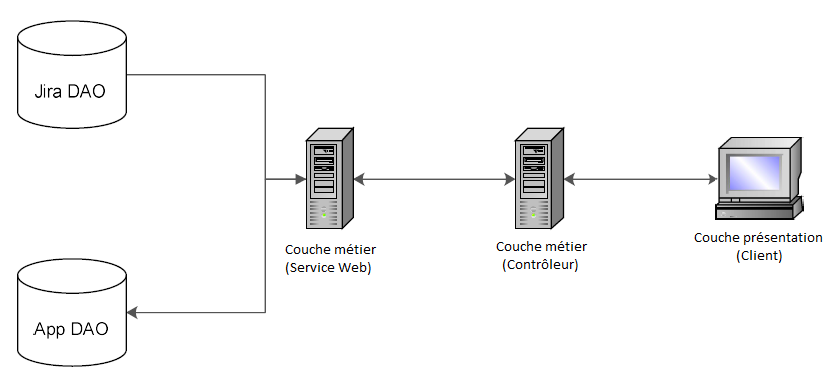
\includegraphics[scale=0.8]{figures/style_architecture.png}
  \caption{Modélisation du système}
  \label{code54}
\end{figure}
\subsection{Pattern architectural}
Un pattern architectural est modèle de référence qui sert à concevoir un système d'information en donnant les sous-systèmes qui le composent , les relations et un ensemble de règles à suivre afin d'organiser les relations entre ces derniers \cite{PatternArchitectural}.
Notre système suit deux patterns architecturaux:\\
\begin{itemize}
    \item[$\bullet$] L’inversion de contrôle (IoC) qui est un pattern architectural qui donne le contrôle du flux d'exécution au framework utilisé. Il existe plusieurs représentations de l'IoC, le framework Spring utilise l'injection de dépendance qui permet de découpler les dépendances entre les objets du projet \cite{IoC}.
    \item[$\bullet$] Modèle - vue - vue modèle (MVVM) qui est un pattern architectural qui permet de séparer entre le modèle et la vue en mettant une vue-modèle comme intermédiaire entre les deux. Ce dernier joue le rôle de convertisseur entre la vue et le modèle. AngularJS utilisent ce qu'on appelle liaison de données (data-binding en anglais) qui permet de modifier la vue si le modèle change et vis versa \cite{MVVM}.\\
\end{itemize}
La figure \ref{code55} présente le pattern architectural de notre application.
\begin{figure}[H]
  \centering
  \includegraphics[scale=0.65]{figures/pattern_diagram.png}
  \caption{Pattern Architectural}
  \label{code55}
\end{figure}
\section{Conclusion}
Dans ce chapitre nous avons présenté l'environnement matériel et logiciel de notre application. Ensuite nous avons détaillé notre style architectural. Et enfin, nous avons présenté le pattern architectural de notre projet. Dans le prochain chapitre, nous allons présenter l'organisation de nos sprints.